\chapter{Einleitung}
%Beschreibe den Hintergrund und die Motivation deiner Arbeit. Erkläre, warum dieses Thema wichtig ist und welche Forschungsfragen du untersuchst.
Das Ziel dieser Abreit ist es ein virtuelle Umgebung zu erstellen um für die Entwicklung von Algorithmen für die sichere Personenerkennung in Automated Guided Vehicle. 
%Verstehe das Problem
Es sollen Umweltdaten von Automated Guided Vehicle Applikationen zur Entwicklung generiert werden. Die Umweltdaten sollen zum testen und Validieren von Sicherheitskonzepten. So sollen Worst-Case-Szenarien definiert werden und die Robustheit der Softwarealgorithemen geprüft werden.\\

Der Vorteil ist es das so viele mehr testdaten generiert werden könne ohne aufwendige Test Scenerien in einer realen Werkshalle aufzubauen.\\
%Identifiziere das Problem
%Hintergrundinformationen
%Relavanz betonen
%Ziele und Hypothesen
%Betonung des Neuigkeitswertes
%Zusammenfassung
%Zusätliche Quellen

%\section{Projektumfeld und Kontext}% kann auch weg gelassen werden
%GICTICIISM
%Global Industry Centers Technical Industry Competence \& Innovation

\section{Problemstellung}
%Verständnis des Themas: Stelle sicher, dass du ein klares Verständnis für das Thema deiner Arbeit hast, bevor du die Problemstellung formulierst.
%Identifikation des Problems: Überlege, welche spezifische Frage oder Herausforderung du in deiner Arbeit angehen möchtest. Welche Lücke in der bestehenden Forschung möchtest du schließen oder welches Problem möchtest du lösen?
%DSM Project was ist dieses Projekt?
Die Problemstellung bindet sich im DSM ein. Es sollen die Sceneie aufgebaut werden und die Sensordaten dem gRPC Server bereitgestellten werden.
\begin{figure}[htp]
    \centering
    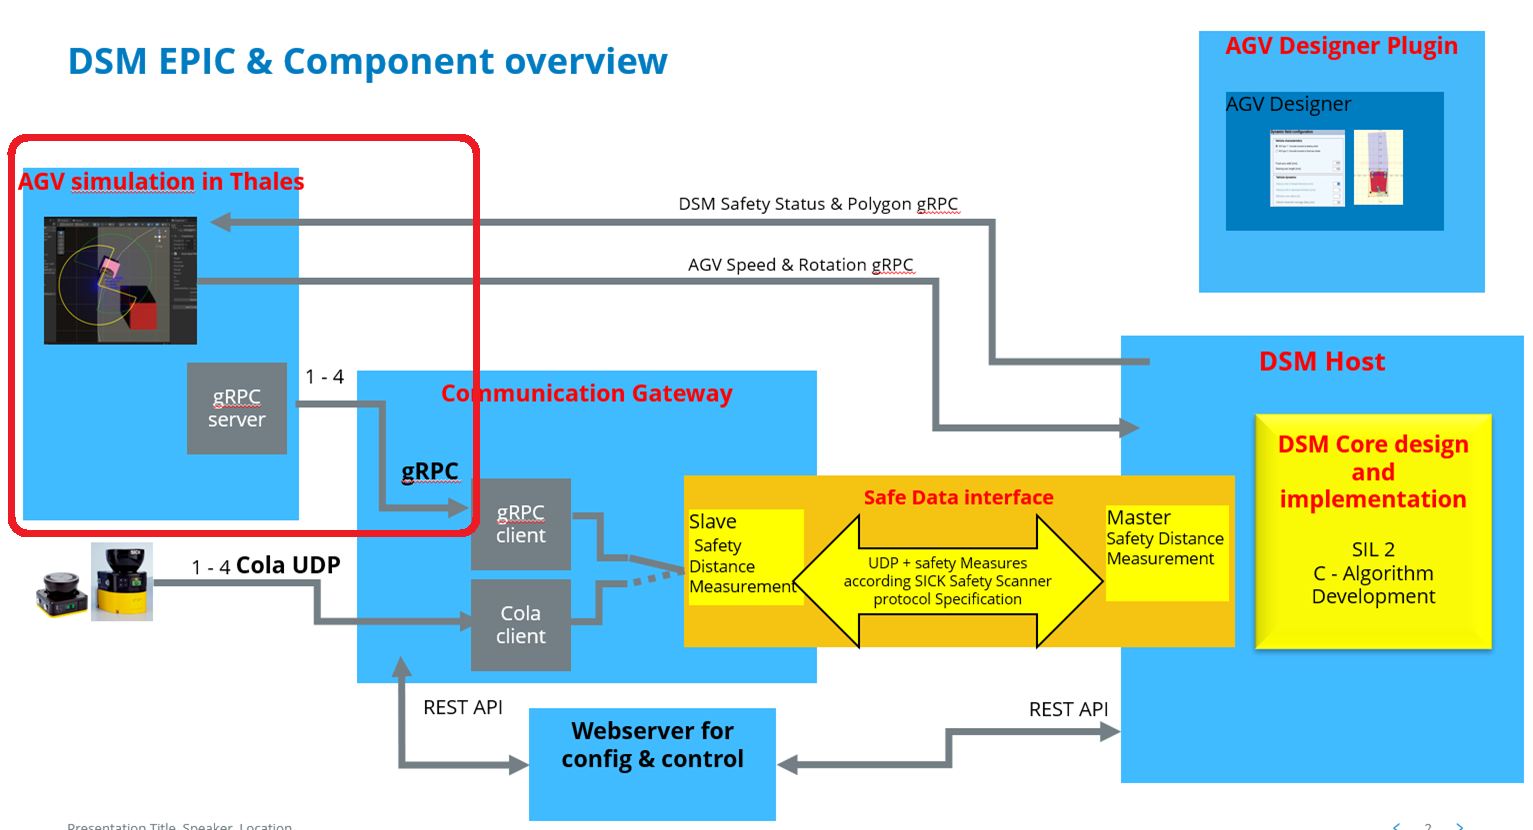
\includegraphics[width=(\textwidth)]{images/AGV_Overview.png}
    \caption{DSM EPIC \& Component overview}
    \label{fig:DSMoverview}
\end{figure}
%Wo finde ich informationen zum DSM Projekt? Boris morgen fragen
%Was trage ich zu deisem Projekt bei?

%Identifiziere die Lücke im Wissen:
Es gib keine Simulation in der man Gefahrensitzuationen testen kann. Ohne Sie in echten Hallen zu testen.
%Spezifische Fragestellung: Formuliere deine Problemstellung als eine klare Frage. Diese Frage sollte präzise, klar und relevant sein. Vermeide vage oder mehrdeutige Formulierungen.


%Bedeutung und Relevanz Betone die Bedeutung deiner Problemstellung. Warum ist es wichtig, diese Frage zu beantworten oder dieses Problem zu lösen? Welche Auswirkungen könnte die Antwort haben?
Im weiteren verlauf kann der Algorithmus der die Sicherheitsfelder der AGVs berechnet an ein Instutut geschickt werden der diesen Valiediert. Oder ein in der Simulation getesten Algorithmus in echten Szenarien getestet werden.
Hier können die Sicherheitsalghrutmen erstmals getestet werden.

%Abgrenzung und Kontext: Kläre den Rahmen deiner Problemstellung. Welche Aspekte deines Themas wirst du behandeln und welche wirst du bewusst außer Acht lassen? Definiere den Kontext, in dem deine Fragestellung relevant ist.


\section{Zielsetzung}
%Die Zielsetzung beschreibt das übergeordnete Ziel deiner Arbeit. Sie verdeutlicht, was du mit deiner Forschung erreichen möchtest.
%Konkretheit: Formuliere deine Zielsetzung so konkret wie möglich. Vermeide allgemeine Formulierungen, die mehrdeutig sind.
%Messbarkeit: Stelle sicher, dass dein Ziel messbar ist. Das bedeutet, dass du später überprüfen können solltest, ob du es erreicht hast.
%Realistisch: Deine Zielsetzung sollte realistisch sein und in einem angemessenen Rahmen erreichbar sein.
%Relevanz: Betone, warum dein Ziel wichtig ist und welche Bedeutung es für die Forschung oder die Praxis hat.
Daten übermittel und ein AGv in Unity erstellen.

\section{Fragestellung}
%Die Forschungsfrage konkretisiert deine Zielsetzung und gibt die Richtung für deine Untersuchung vor. Sie sollte präzise, klar und offen genug sein, um die Möglichkeit zur Forschung zu bieten.
%Klarheit: Formuliere die Forschungsfrage klar und verständlich. Vermeide komplexe Satzstrukturen.
%Ein Frageaspekt: Fokussiere auf einen bestimmten Aspekt des Themas. Eine zu breite Fragestellung kann zu unübersichtlichen Ergebnissen führen.
%Beantwortbarkeit: Stelle sicher, dass deine Forschungsfrage durch deine Forschungsmethoden und Daten beantwortbar ist.

Wie kann ein AGV in Unity in erstellt werden und dessen Meschanische Daten über gRPC mit der Ausenwelt geteilt werden und auch Daten erhalten? 